\label{sec::theory}
\subsection{State of the Art}
% Review all of the current experimental evidence pertaining to my area of research
%\todo[inline]{Talk quantum electron spin, projective measurement vs non-projective measurement (bloch sphere), about technology behind SETs}
\subsubsection{Quantum Information}
	\todo[inline]{Make this less terrible.}
	A quantum computer is composed of quantum bits of information, known as qubits. The difference between a classical bit and a quantum bit is the concept of quantum entanglement. Where any classical bit can be read and written independently of other bits in the system, the same cannot always be said of quantum bits. Reading or writing to a qubit can cause other entangled qubits in the system to change, as a single qubit no longer has a defined binary state, but it can be in a superposition of a logical "1" or "0" state. This superposition increases the information density of a quantum system, and to represent a fully entangled n-qubit system in a classical computer requires $2^n$ bits. \cite{bennett2000quantum}
	
	In the devices manufactured by \gls{cqc2t}, a qubit is created from the physical property of an electron known as spin. Spin is the intrinsic magnetic moment of nano structures, essentially a small magnetic dipole, that can point in any direction in free space. For an electron, you can measure the value of this magnetic moment to be $S = \frac{\hbar}{2}$ (denoted "spin one half"). Despite this freedom of orientation, if you were to measure this spin in an arbitrary orientation, you will always find the spin to be aligned or anti-aligned to the axis of measurement (with some exceptions). For example, if you were to measure in the z-axis you would find the following:
	$$S_x = 0; S_y = 0; S_z = \pm\frac{\hbar}{2}$$
	
	where the sign indicates alignment or anti-alignment.
	
	This means that spin qubits can only be observed in one of two possible states at a time. These states are named "spin-up" or "spin-down", which corresponds to the north pole pointing up or down, respectively, with regards to the axis of measurement (typically the vertical z-axis). A single readout is not enough to determine the complete state of a qubit, and an average must be taken over many samples to determine the true state. \\
	
	\label{zeeman}
	If you apply an external magnetic field to these spins, you introduce an energy difference between the spin-up and spin-down states, known as the Zeeman splitting. Using this energy difference, we can perform a spin-dependent readout from a special device, introduced in the next section. It's important to note that this energy difference is much smaller than the thermal energy of a typical room, so all experiments are performed at cryogenic temperatures, ranging from 4K to less than 100 mK. \cite{morello2010single}
	
\subsubsection{Quantum Devices}
	\label{sec::set}
	A quantum device is any device that operates on the principles of quantum mechanics. An example is a \gls{set}, where the simplest variety can be described using the equivalent electrical circuit \cite{devoret2000amplifying} shown in Figure \ref{fig::set_circuit}. The components between the source and drain are called tunnel junctions, which can allow electrons to travel through them, even if the energy of the barrier is higher than the energy of the electron. Due to the arrangement of these components, an island is formed between each node of the typical FET transistor, which is coupled to the gate capacitively and to the drain and source through the tunnel junctions, but it is otherwise electrically isolated from the rest of the system.
	
	Due to the isolation of the island, the only way for it to gain or lose a charge is through the drain or source. However, due to the capacitive coupling to the gate through $C_G$, energy is required to increase the charge of the island (assuming $V_G$ is constant), and as the energy of the island is given by $$E_C = \frac{Q^2}{2 C_\Sigma} ; C_\Sigma = C_D + C_S + C_G$$ we can define a quantity known as the charging energy of the capacitor. Adding or removing a single electron from the island would require an energy $\Delta E = \frac{e^2}{2 C}$ which can be on the order of 1 meV. This energy describes the difference in potential created by moving an electron from infinitely far away to on the island, though much smaller charge differences are realisable, and a charge-continuum is formed when the dielectric charge is accounted for.
	
	
	
	
	
	Figure \ref{fig::coulomb_blockade}, shows the relationship between the potential energy of the island and conductance through the drain-source. The upper diagram shows all lower energy states are filled, and thus no electron can pass from the source to the island. If we then raise the island potential up, akin to lowering the gate voltage
	 (we assume at this point that the gate capacitor does not discharge), 
	 we have created an allowable energy level that can be filled from the source, and can then later tunnel to the drain. While the electron is on the island, there are no further available energy states and thus, we have created a transistor which will only allow a single electron to pass from source to drain at a time.
	
	\begin{figure}[htbp!]
		\centering
		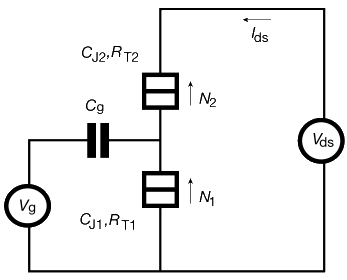
\includegraphics[width=0.6\textwidth]{set_circuit}
		\caption[Equivalent circuit of an \gls{set}]{Equivalent electrical circuit of an \gls{set}\cite{devoret2000amplifying}}
		\label{fig::set_circuit}
	\end{figure}
	
	\begin{figure}[htbp!]
		\centering
		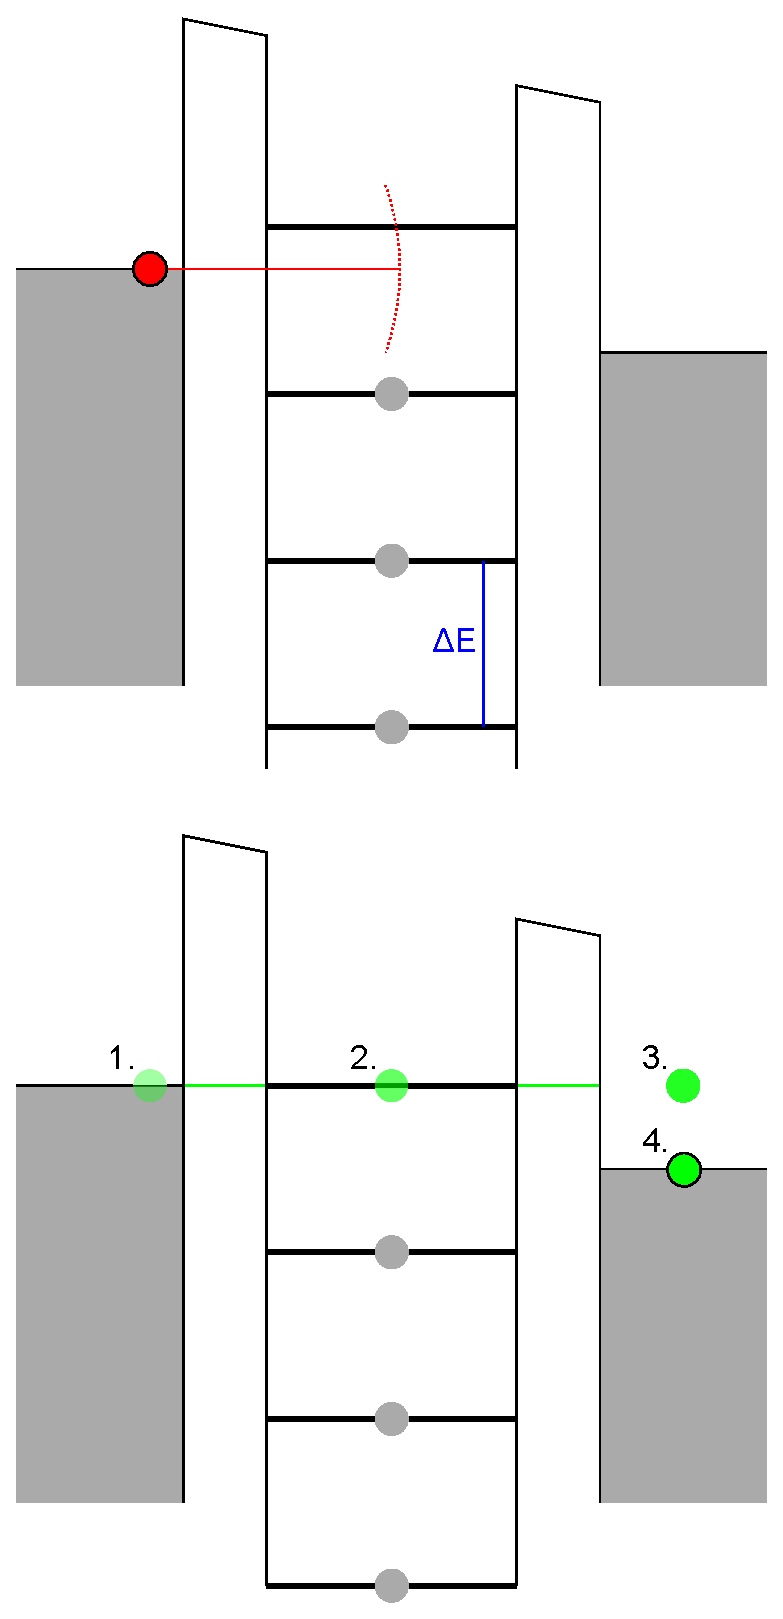
\includegraphics[width=0.6\textwidth, height=0.8\textheight]{coulomb_blockade}
		\caption[A Coulomb Blockade]{A Coulomb Blockade \cite{coulomb_blockade} forms due to electrostatic potential difference between island and source.\\ In the upper diagram, all allowable energy states are below the Fermi energy of the reservoir, hence no transmission can occur.\\ In the lower diagram, the potential of the quantum well has been raised, and now an empty state can be occupied by an electron from the source, which will subsequently tunnel off to the drain.}
		\label{fig::coulomb_blockade}
	\end{figure}
	
	\begin{figure}[htbp!]
		\centering
		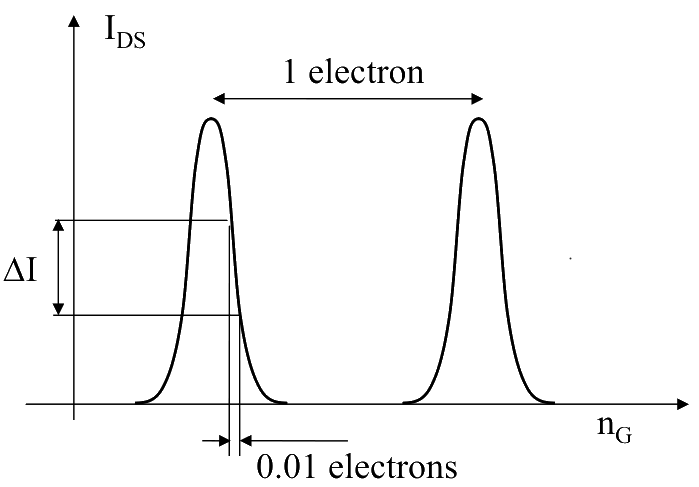
\includegraphics[width=0.8\textwidth]{coulomb_peaks}
		\caption[Coulomb Peaks]{Coulomb Peaks form due to the discrete energy levels allowed on the island\cite{elec9705_lecture}}
		\label{fig::coulomb_peaks}
	\end{figure}
	
	
	%\todo[inline]{Talk about spin dependent tunnelling}
	
	Recalling the Zeeman splitting energy (Section \ref{zeeman}) that is created through the application of an external magnetic field, if we can then shift the average energy level of an electron, we can allow the higher energy state to be transmitted through the coulomb blockade, while the lower energy state will not be transmitted \todo[inline]{This is misleading, coulomb blockade is due to the presence/absence of an electron on the gate in our setup.}. This is known as spin-dependent tunneling, and in silicon, the higher energy state is spin up. This is depicted in Figure \ref{fig::set_loading}, where diagram b shows the Fermi level in green, and the red and blue lines are the energy levels of a spin-up and spin-down electron, respectively. 
	
	Furthermore, what we see when the coulomb blockade is lifted is a defined current through the \gls{set} from drain to source. This current is due to the sudden polarization of the phosphorus donor in silicon, as an electron tunnels off of the donor, into a reservoir. This positive voltage can shift the island voltage to allow for a larger \gls{set} current to flow, referring to Figure \ref{fig::coulomb_peaks} which shows the SET current as a function of gate charge, until an electron rejoins the phosphorus donor. This larger current is used to indicate the electron spin state, as ideally only a spin-up electron will tunnel off of the donor.
	
	\begin{figure}[htbp!]
		\centering
		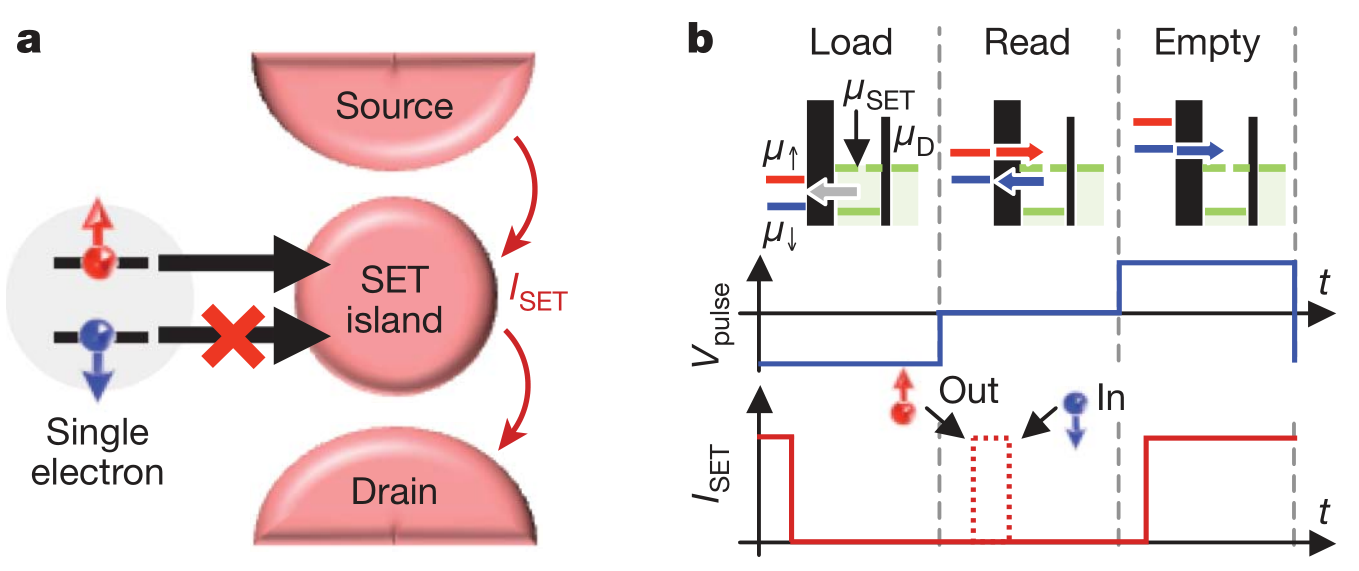
\includegraphics[width=\textwidth]{set_loading}
		\caption[The initiliasation prodedure]{The initialisation procedure of an \gls{set}\cite{morello2010single}}
		\label{fig::set_loading}
	\end{figure}
	
\subsection{Quantum Control}
	\subsubsection{Hyperfine Interaction}
		In this thesis, we are considering a single $^{31}$P donor implanted near the \gls{set} island. This donor has a single unbound electron on which we can perform spin operations, this will be explored in the next section. The phosphorus donor nucleus is also a spin-half particle, and due to its proximity with the donor electron, there is a magnetic interaction which acts as an extra magnetic source which splits the energy levels.
		\todo[inline]{Put a diagram here explaining the energy splitting}
		
		By modulating the gate voltages, we shift the electrostatic environment about the donor, and hence we change the coupling between the donor nucleus and electron. This in turn modifies the hyperfine interaction, and therefore changes the energy splitting. This change in coupling can be thought of as due to the distance between the electron and nucleus.
		\todo[inline]{Improve this, talk about resonance shift}
		
		By tuning our gate voltages and keeping them steady, we can search for the resonance frequency for both our nucleus and electron. 
	\subsubsection{Nuclear and Electron Spin Mapping}
	\label{sec::nuc_spin_map}
	\todo[inline]{Discuss NMR/ESR and the state evolution}
	\todo[inline]{specifically explain NMR}
		We can translate an energy difference into a frequency of an electromagnetic wave using $E = h f$, which means we can affect a state transition by applying a microwave or radio frequency pulse.
		
		By mapping the electron spin state to the nucleus we can increase the coherence time of our measurements, as the nucleus is more immune to perturbations in the environment than an electron. Consider Figure \todo[inline]{insert figure showing 4 energy states here}
		
		We can map an electron state to the nucleus by first initialising the electron to a known state, in our case spin down, then performing the desired operations, followed by a mapping operation, such as a CNOT or SWAP gate.
		\todo[inline]{Explain more about mapping}
		
	\subsubsection{Quantum Steering of an Electron Spin}
	
	When the plunger is at the readout position, ideally a spin up electron would be able to tunnel off, and a spin down electron will be able to tunnel back on. However, due to the non-zero ambient temperature, we find that the Fermi distribution becomes bent, and there are allowable energy states below the Fermi level, and there are occupied states above the Fermi level. These are depicted in Figure \ref{fig::errors}, where the read error $(\alpha)$ indicates that we would read a blip in current incorrectly as a spin-up electron being present on the donor. Similarly, the load error $(\beta)$ is when an electron is allowed to tunnel onto the donor from the reservoir, and it is this error which I am trying to minimise. To understand how to minimise this error, we must understand the concept of electron spin steering.
	
	\begin{figure}[htbp!]
		\centering
		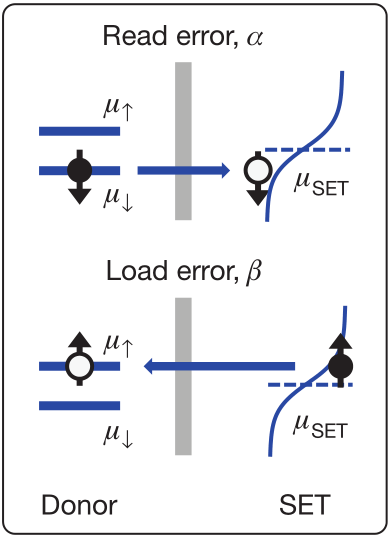
\includegraphics[height=0.3\textheight]{readout_errors}
		\caption[Load and red errors in the \gls{set} readout position]{Load and read errors that occur when the \gls{set} is in the readout position.\cite{electron_spin_silicon}}
		\label{fig::errors}
	\end{figure}
	
	Once the island has been shifted to the readout position, an electron does not simply tunnel off immediately. There is an average tunnel time associated with the characteristics of the tunnel junction, namely the tunnel resistance and the junction capacitance. The probability of an electron tunnelling through a tunnel junction exponentially decays over time, meaning it is more likely for an electron to leave sooner, rather than later. \\
	
	\todo[inline]{Fix this!!}
	Suppose the average tunnel time $(\tau)$ of an electron is 1 ms, and suppose we had an electron with an unknown spin loaded onto the donor, and we observe the state for a time much shorter than $\tau$, say 1 $\mu$s. If no tunnel event occurs, this is not indicative that the electron would not tunnel in the future, and so we have only gained a small amount of certainty of the state of the electron. In reality, we cannot know an electron spin state with complete certainty unless we were to wait for an infinite amount of time, but by waiting longer periods of time, we gradually gain more information about the state. If a tunnel event occurs, we know for that instance the electron was spin up. However, if no tunnel event occurs for a time T; the likelihood that the electron is spin down increases proportional to $1-\exp\left(-\frac{T}{\tau}\right)$. \todo[inline]{how to express this truly as proportional... it's basically equivalent} This process is known as weak measurement, as we gradually gain more information about the system, which is different from a strong, or projective, measurement which gives an exact value at that point in time. Figure \ref{fig::spin_readout_decay} expresses this concept pictorially, after an arbitrarily spin-aligned electron joins the donor, the current readout drops, though the probability of the electron being spin up is still 50\% due to the load error shown in figure \ref{fig::errors}, over time this decays to 0\%. 
	
	With this information, there are 3 possibilities in initializing a spin-qubit, which are shown in Figure \ref{fig::init_possibilities}. The first plot shows the trivial case of no tunnel event occurring for a long time, indicating the loaded spin is spin-down. The middle plot shows an adequate amount of time between the plunge time and the last current blip, which presents the case for improving spin initialization. The bottom plot shows the worst case scenario, where the donor was plunged with no electron. This would result in a completely randomised spin, yielding unusable results. 
	
	\begin{figure}[htbp!]
		\centering
		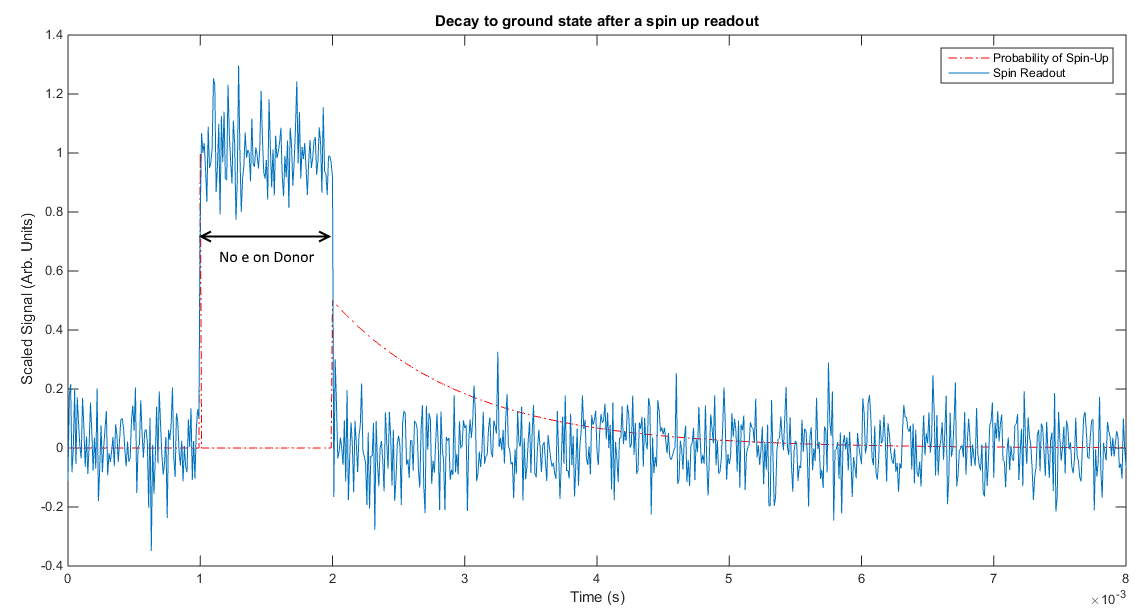
\includegraphics[width=\textwidth]{spin_readout_decay}
		\caption{Electronic Spin Steering}
		\label{fig::spin_readout_decay}
	\end{figure}
	
	\begin{figure}[htbp!]
		\centering
		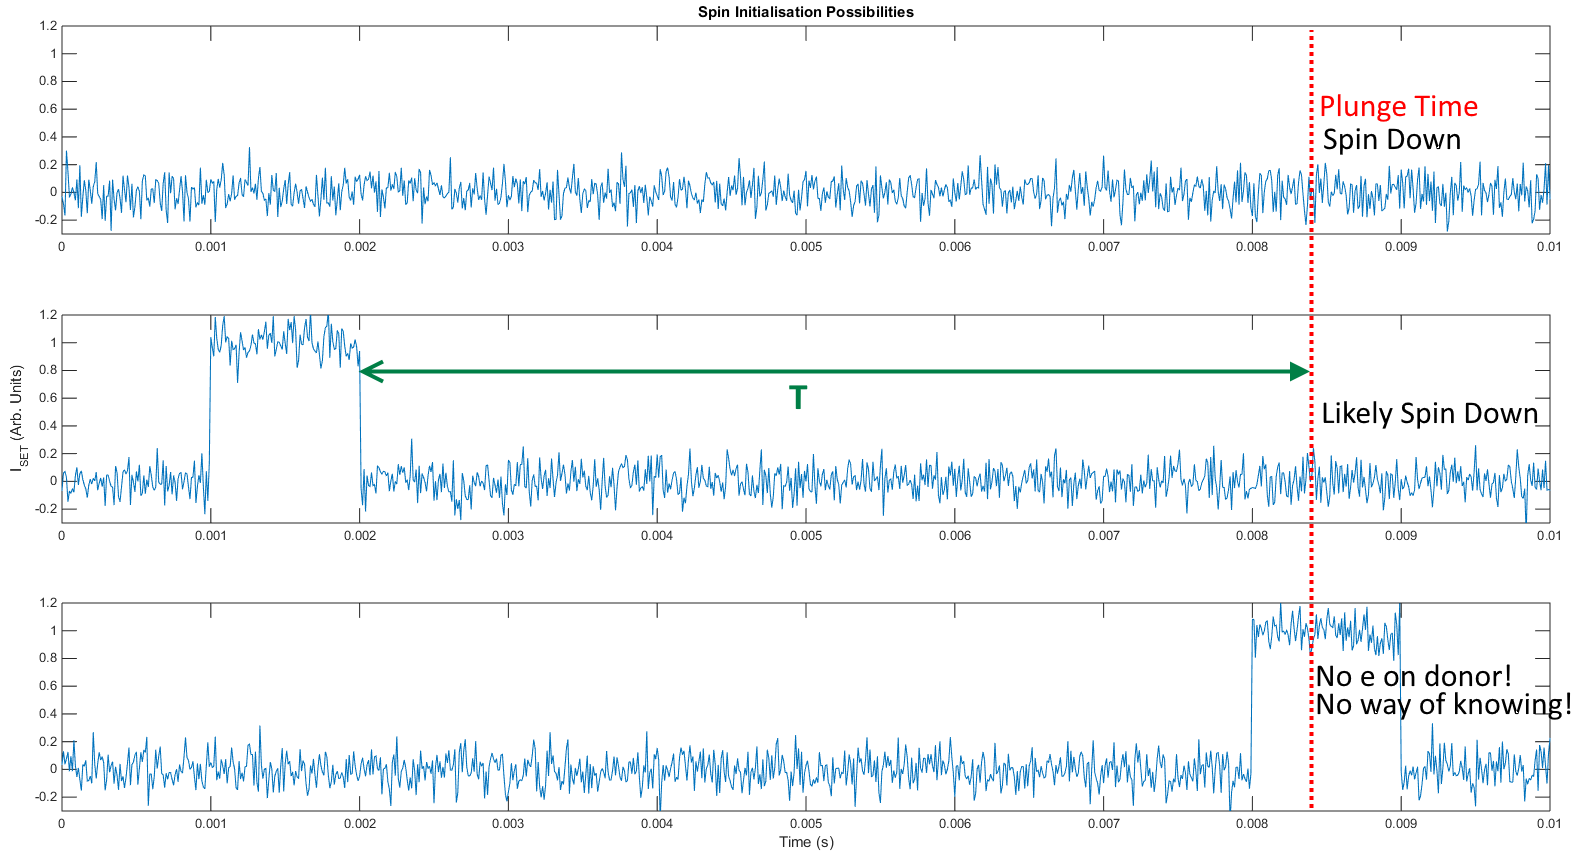
\includegraphics[width=\textwidth]{init_possibilities}
		\caption[Possible initialisation outcomes]{Possible intialization outcomes: Spin-down initialization is favourable, thus plots become decreasingly desirable from top to bottom.}
		\label{fig::init_possibilities}
	\end{figure}
	
	Figures \ref{fig::spin_steering} and \ref{fig::spin_steering_log} show the exponential decay function. Using this function, we can determine an adequate amount of time to wait to achieve a 99.9\% initialisation fidelity is $7 \tau$. For reference, $5 \tau$ and $3 \tau$ will yield an initialisation fidelity of 99.7\% and 97.5\% respectively.
	
	\begin{figure}[htbp!]
		\centering
		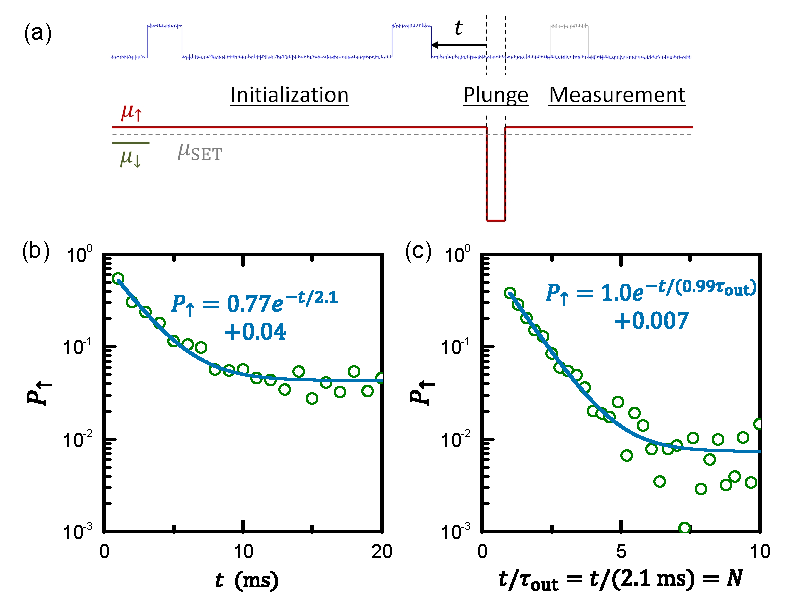
\includegraphics[width=\textwidth]{rach_steering}
		\caption[Initialisation fidelity with varying steering times, via post-selection.]{Initialisation fidelity with varying steering times, obtained via post-selection.
			(a) data points were binned based on the time $t$ from the time of plunge. 
			(b) direct readout is performed from the electron after returning from plunge.
			(c) readout is performed after mapping the electron spin to the nucleus, and then performing several subsequent electron readouts, mapped from the nucleus spin.
			\cite{rachpon_thesis}}
		\label{fig::rach_steering}
	\end{figure}
	
	
	\begin{figure}[htbp!]
		\centering
		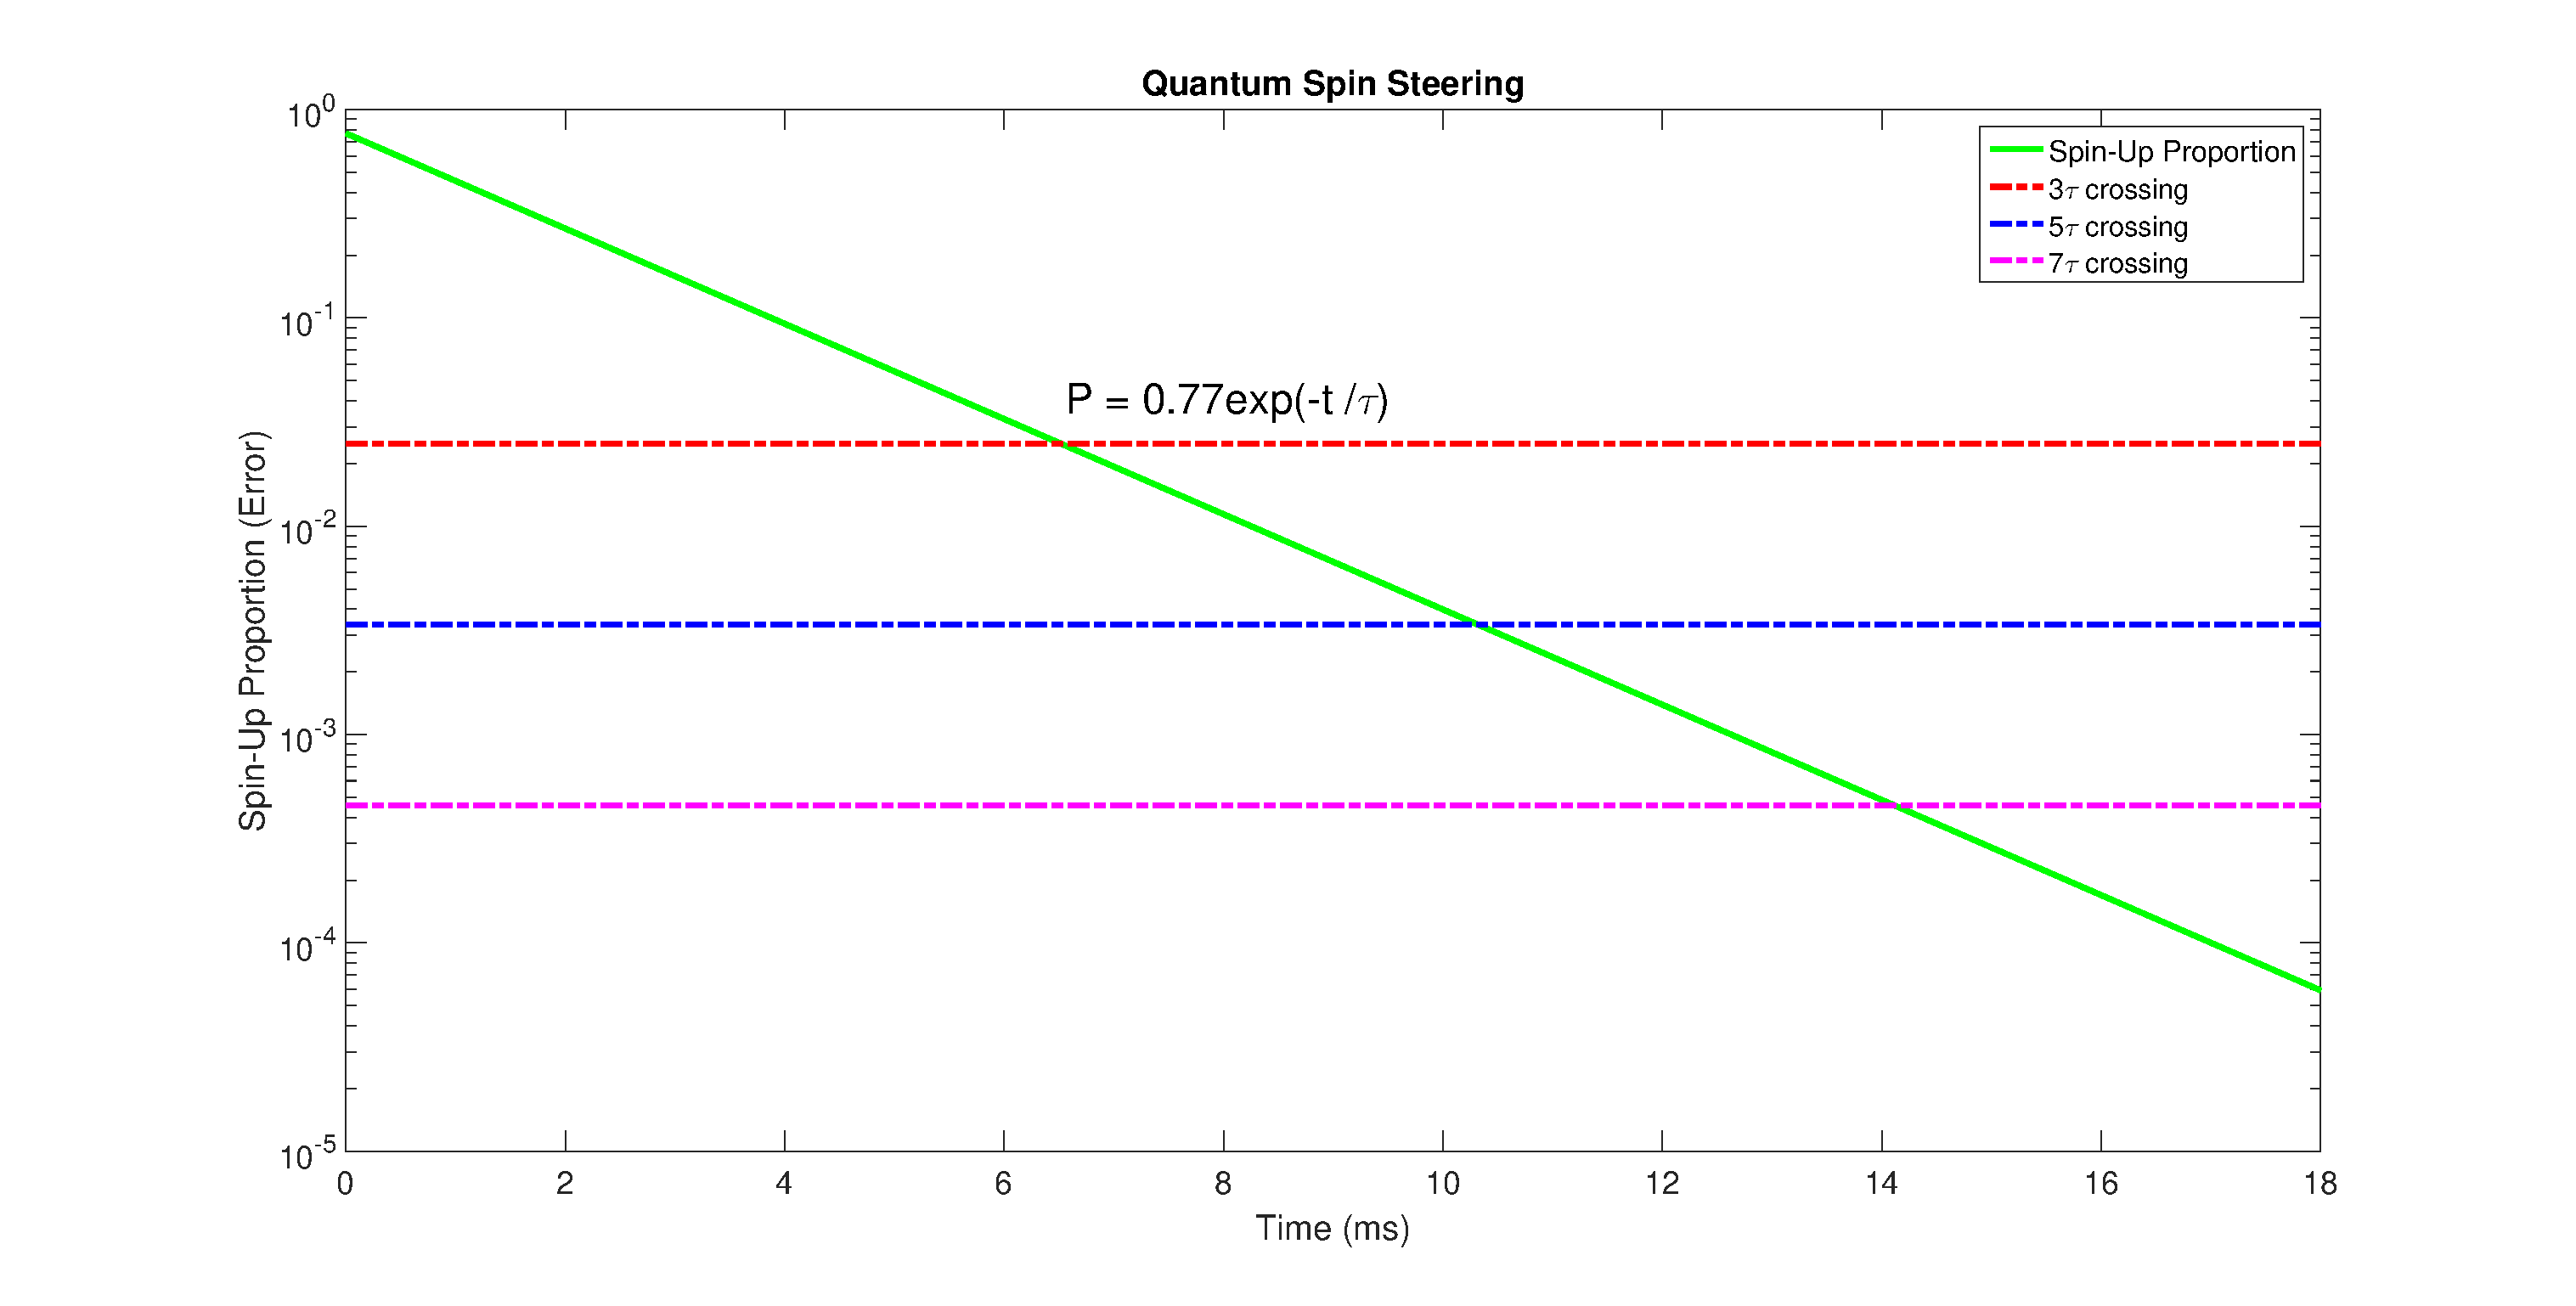
\includegraphics[width=\textwidth]{steering_log}
		\caption{Close up of Figure \ref{fig::spin_steering}, semilog plot to show P versus multiples of $\tau$}
		\label{fig::spin_steering_log}
	\end{figure}

\subsubsection{Electron Spin Initialisation}
\label{sec::spin_init}
\todo[inline]{Cite Rachpon's thesis, discuss here}
Previous research \cite{rachpon_thesis} has quantified an improvement in qubit control when initialisation fidelities are increased. Figure \ref{fig::rach_steering} depicts results that were gathered using post-selection on a repeated sequence shown in sub-plot (a). The sequence was to move to the initialisation level for 20 ms, and then plunged for 1 ms to cease steering, and finally it is moved to the readout level to observe the state of the electron spin. This was repeated 40,000 times to obtain statistics. 

The results showed that steering does increase based on the time spent steering, until a floor is reached, which is shown in the model applied to both sub-plots (b) and (c). The error floor was 4\% and 0.7\%, respectively, which indicates the best achievable fidelity for this particular configuration was 99.3\%.

\begin{figure}[htbp!]
	\centering
	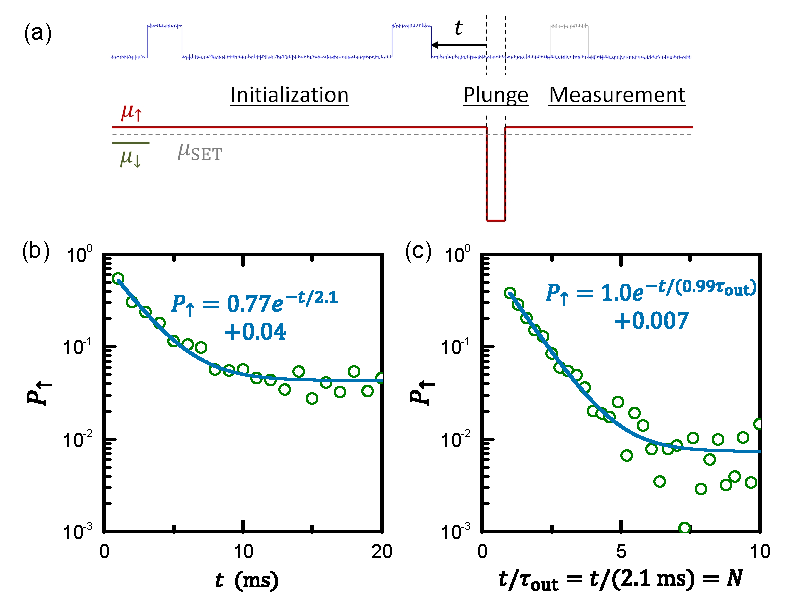
\includegraphics[width=\textwidth]{rach_steering}
	\caption{Initialisation fidelity with varying steering times, obtained via post-selection.
		(a) data points were binned based on the time $t$ from the time of plunge. 
		(b) direct readout is performed from the electron after returning from plunge.
		(c) readout is performed after mapping the electron spin to the nucleus, and then performing several subsequent electron readouts, mapped from the nucleus spin.
		\cite{rachpon_thesis}}
	\label{fig::rach_steering}
\end{figure}

Further work was undertaken which improved fidelities by fine-tuning the electrochemical potentials, to ensure that the vast majority of tunnel events will be observed, and not hidden by the finite amplifier bandwidth of the experiment. Under this tuning, repeating the same task of binning readouts based on the amount of time spent steering before a plunge.

\todo[inline]{Introduce Rachpon's thesis, its contributions, and the breadth of knowledge known so far}
\todo[inline]{Engage in the initialisation section, and discuss the effects of improving this fidelity on the rest of the experiment, in particular, take note of the ability to also perform the nuclear spin readout as a method of minimizing readout error. Combining these two things together, as well as gate fidelities, we have an overall high fidelity system.	I may want to describe/quantify the overall system fidelity, as a product (?) of the other fidelities.}


\subsubsection{Digital Feedback in Quantum Devices}

%\todo[inline]{Talk about the place of digital feedback in quantum systems}
%\todo[inline]{find more digital feedback stuff}
Digital feedback has recently been explored in the development of a quantum computer. For example, it has been used to reduce error in resonance estimation \cite{bonato2015optimized} and increase coherence time of a single qubit through adjusting control parameters \cite{shulman2014suppressing}. As such, it is likely to be a key factor in the future of quantum computers, especially once they are realised as black-box systems.
